% this is the main file for each individual chapter
% each chapter has a subfolder, which contains a main.tex that simply inlines this file

\ifx\synctex\undefined\else\synctex=1\fi

\documentclass[b5paper,11pt]{book}

\usepackage[utf8]{inputenc}
%% (FMu) uzywamy \lw do napisania l z kreska, bo potem cos
%% przedefiniowuje \l na \lambda. To nie jest eleganckie,
%% ale dziala. To samo dla czeskiego hacka (np. w Cerny)
\let\lw\l  
\let\hacek\v

\usepackage{amsfonts}
\usepackage[fleqn]{amsmath} %fleqn does left allignment of display formulas
\usepackage{amssymb,amsmath}
\usepackage{amsthm}
\usepackage{graphicx}
\usepackage{xspace}
\usepackage{todonotes}
\usepackage{mathbbol}
\usepackage{enumerate}
\usepackage{comment}
\usepackage{enumitem}
\usepackage{hyperref}
\usepackage{bookmark}
\usepackage{nameref}
\usepackage{ifthen}
\usepackage{algorithm}
\usepackage[noend]{algpseudocode}
\usepackage{tikz}
\usepackage[normalem]{ulem}
\usepackage[all]{xy}
% \usepackage{mdframed} 
\usepackage{fancyhdr}
\usepackage{pdfpages}
\usepackage{mathtools}


\RequirePackage[osf,sc]{mathpazo}
\usepackage[mathcal]{euscript}



%style


\newcommand{\views}{\mathsf{views}}

\pagestyle{fancy}

\newcommand{\period}{.}%used in equations
\newcommand{\comma}{,}%used in equations

\newcommand{\tn}[1]{#1}% a number which is inlined in the text, and could be replaced by a word, e.g.
%has length at most \tn{3}
\newcommand{\an}[1]{$#1$}% a number which is inlined in the text, but represents an alphabet symbol,
%e.g. the set of words in which the number of \an{1}'s and \an{0}'s are equal.

%shrink bullets
\newlength{\mylen}
\newlength{\itemizemargin}%leftmargin for itemize lists
\newlength{\itemizelabelsep}%labelsep for itemize lists
\setbox1=\hbox{$\bullet$}\setbox2=\hbox{\tiny$\bullet$}
\setlength{\mylen}{\dimexpr0.5\ht1-0.5\ht2}
\setlength{\itemizemargin}{27pt}
\setlength{\itemizelabelsep}{\dimexpr 0.4\itemizemargin}
\renewcommand\labelitemi{\raisebox{\mylen}{\tiny$\bullet$}}
\renewcommand\labelitemii{\raisebox{\mylen}{\tiny$\bullet$}}
\setlist[itemize]{leftmargin=\itemizemargin,labelsep=\itemizelabelsep}

\newcommand{\tagsymbol}{$\diamond$}


\DeclareTextFontCommand{\textsmallcaps}{\scshape}

      \RequirePackage{letterspace}
      \RequirePackage{textcase}
      % Set up letterspacing (using microtype package) -- requires pdfTeX v1.40+
      \newcommand{\allcapsspacing}[1]{\textls[200]{#1}}
      \newcommand{\smallcapsspacing}[1]{\textls[50]{#1}}
      \newcommand{\allcaps}[1]{\textls[200]{\MakeTextUppercase{#1}}}
      \newcommand{\smallcaps}[1]{\smallcapsspacing{\scshape\MakeTextLowercase{#1}}}
      \renewcommand{\textsc}[1]{\smallcapsspacing{\textsmallcaps{#1}}}

\newcommand{\newlinetospace}[1]{#1}
% \DeclareRobustCommand{\newlinetospace}[1]{%
%   \let\@tufte@orig@cr\\% save the original meaning of \\
%   \def\\{\@tufte@newlinetospace}% turn \\ and \\* into \space
%   \let\newline\\% turn \newline into \space
%   #1%
%   \let\\\@tufte@orig@cr% revert to original meaning of \\
% }

\makeatletter
\newcommand*{\currentname}{\@currentlabelname}


\newcommand\iraggedright{%ragged right with indentation
  \let\\\@centercr\@rightskip\@flushglue \rightskip\@rightskip
  \leftskip\z@skip}



\newboolean{@test@}%if true, only parts encompassed in environment testshow will be typeset.
\setboolean{@test@}{true}

\newcommand{\testhide}[1]{
\ifthenelse{\boolean{@test@}}{}{#1}%in test mode contents is hidden
}


\newboolean{@tufte@symmetric}
\setboolean{@tufte@symmetric}{true}
\newboolean{@tufte@twoside}
\setboolean{@tufte@twoside}{true}


% The running heads/feet don't have rules
\renewcommand{\headrulewidth}{0pt}
\renewcommand{\footrulewidth}{0pt}
\newcommand{\plaintitle}{}
\newcommand{\plainauthor}{}
\setlength{\headsep}{45pt}
% The 'fancy' page style is the default style for all pages.
\fancyhf{} % clear header and footer fields
\newcommand{\headdisplay}[1]{{\fontsize{6.5}{0}\fontseries{b}\selectfont\scshape\textls[150]{#1}}}
\fancyhead[LE]{\thepage\quad\headdisplay{\leftmark}}%
\fancyhead[RO]{\headdisplay{\rightmark}\quad\thepage}


\renewcommand{\chaptermark}[1]%
   {\markboth{\MakeUppercase{#1}}{}}
\renewcommand{\sectionmark}[1]%
   {\markright{\MakeUppercase{#1}}}


\newlength{\@tufte@overhang}% used by the fullwidth environment and the running heads
\newlength{\@tufte@fullwidth}
\newlength{\@tufte@caption@fill}

\newcommand{\TufteRecalculate}{%
  \setlength{\@tufte@overhang}{\marginparwidth}
  \addtolength{\@tufte@overhang}{\marginparsep}

  \setlength{\@tufte@fullwidth}{\textwidth}
  \addtolength{\@tufte@fullwidth}{\marginparsep}
  \addtolength{\@tufte@fullwidth}{\marginparwidth}

  \setlength{\@tufte@caption@fill}{\textwidth}
  \addtolength{\@tufte@caption@fill}{\marginparsep}
}

\AtBeginDocument{\TufteRecalculate}
% Set the header/footer width to be the body text block plus the margin
% note area.
% \AtBeginDocument{%
%   \ifthenelse{\boolean{@tufte@symmetric}}
%     {\fancyhfoffset[LE,RO]{\@tufte@overhang}}
%     {\fancyhfoffset[RE,RO]{\@tufte@overhang}}
% }


\RequirePackage{titlesec,titletoc}
%%
% Make Tuftian-style section headings and TOC formatting

\titleformat{\part}%
  [display]% shape
  {\relax\ifthenelse{\NOT\boolean{@tufte@symmetric}}{\begin{fullwidth}}{}}% format applied to label+text
  {}%{\scshape \LARGE part\ \thepart\\}% label
  {0pt}% horizontal separation between label and title body
  {\Huge\rmfamily\itshape}% before the title body
  [\ifthenelse{\NOT\boolean{@tufte@symmetric}}{\end{fullwidth}}{}]% after the title body

\titleformat{\chapter}%
  [display]% shape
  {\relax\ifthenelse{\NOT\boolean{@tufte@symmetric}}{\begin{fullwidth}}{}}% format applied to label+text
  {\itshape\huge\thechapter}% label
  {0pt}% horizontal separation between label and title body
  {\huge\rmfamily\itshape}% before the title body
  [\ifthenelse{\NOT\boolean{@tufte@symmetric}}{\end{fullwidth}}{}]% after the title body


\titleformat{\section}%
  [hang]% shape
  {\normalfont\Large\itshape}% format applied to label+text
  {\normalfont\Large\itshape\thesection}% label
  {1em}% horizontal separation between label and title body
  {}% before the title body
  []% after the title body

\titlespacing*{\chapter}{0pt}{50pt}{40pt}
\titlespacing*{\section}{0pt}{3.5ex plus 1ex minus .2ex}{2.3ex plus .2ex}
\titlespacing*{\subsection}{0pt}{3.25ex plus 1ex minus .2ex}{1.5ex plus.2ex}


%%
% When \cleardoublepage is called, produce a blank (empty) page -- i.e.,
% without headers and footers
\def\cleardoublepage{\clearpage\if@twoside\ifodd\c@page\else
  \hbox{}
  %\vspace*{\fill}
  %\begin{center}
  %  This page intentionally contains only this sentence.
  %\end{center}
  %\vspace{\fill}
  \thispagestyle{empty}
  \newpage
  \if@twocolumn\hbox{}\newpage\fi\fi\fi}

%%
% Set the font sizes and baselines to match Tufte's books
\renewcommand\normalsize{%
   \@setfontsize\normalsize\@xpt{14}%
   \abovedisplayskip 10\p@ \@plus2\p@ \@minus5\p@
   \abovedisplayshortskip \z@ \@plus3\p@
   \belowdisplayshortskip 6\p@ \@plus3\p@ \@minus3\p@
   \belowdisplayskip \abovedisplayskip
   \let\@listi\@listI}
\normalbaselineskip=14pt
\normalsize
\renewcommand\small{%
   \@setfontsize\small\@ixpt{12}%
   \abovedisplayskip 8.5\p@ \@plus3\p@ \@minus4\p@
   \abovedisplayshortskip \z@ \@plus2\p@
   \belowdisplayshortskip 4\p@ \@plus2\p@ \@minus2\p@
   \def\@listi{\leftmargin\leftmargini
               \topsep 4\p@ \@plus2\p@ \@minus2\p@
               \parsep 2\p@ \@plus\p@ \@minus\p@
               \itemsep \parsep}%
   \belowdisplayskip \abovedisplayskip
}
\renewcommand\footnotesize{%
   \@setfontsize\footnotesize\@viiipt{10}%
   \abovedisplayskip 6\p@ \@plus2\p@ \@minus4\p@
   \abovedisplayshortskip \z@ \@plus\p@
   \belowdisplayshortskip 3\p@ \@plus\p@ \@minus2\p@
   \def\@listi{\leftmargin\leftmargini
               \topsep 3\p@ \@plus\p@ \@minus\p@
               \parsep 2\p@ \@plus\p@ \@minus\p@
               \itemsep \parsep}%
   \belowdisplayskip \abovedisplayskip
}
\renewcommand\scriptsize{\@setfontsize\scriptsize\@viipt\@viiipt}
\renewcommand\tiny{\@setfontsize\tiny\@vpt\@vipt}
\renewcommand\large{\@setfontsize\large\@xipt{15}}
\renewcommand\Large{\@setfontsize\Large\@xiipt{16}}
\renewcommand\LARGE{\@setfontsize\LARGE\@xivpt{18}}
\renewcommand\huge{\@setfontsize\huge\@xxpt{30}}
\renewcommand\Huge{\@setfontsize\Huge{24}{36}}

\makeatother


\renewcommand\qedsymbol{\scalebox{0.75}{$\blacksquare$}}

\fancypagestyle{plain}{
  \fancyhf{} % clear header and footer fields
  % Uncomment the following five lines of code if you want the opening page
  % of the chapter to express the folio in the lower outside corner.
  %\ifthenelse{\boolean{@tufte@twoside}}
  %  {\fancyfoot[LE,RO]{\thepage}}
  %  {\fancyfoot[RE,RO]{\thepage}}
}


  \titlecontents{part}%
    [3em] % distance from left margin
{\addvspace{3pt}\vspace{1.5\baselineskip}\LARGE\bfseries\itshape} % above (global formatting of entry)
    {\hspace*{0em}\contentslabel{2em}} % before w/label (label = ``2'')
    {\hspace*{0em}} % before w/o label
    {\rmfamily\upshape\qquad\thecontentspage} % filler + page (leaders and page num)
    [\vspace{5pt}] % after


  \titlecontents{chapter}%
    [3em] % distance from left margin
{\addvspace{3pt}\vspace{1.5\baselineskip}\LARGE\rmfamily\itshape} % above (global formatting of entry)
    {\hspace*{0em}\contentslabel{2em}} % before w/label (label = ``2'')
    {\hspace*{0em}} % before w/o label
    {\rmfamily\upshape\qquad\thecontentspage} % filler + page (leaders and page num)
    [\vspace{5pt}] % after

  \titlecontents{section}% FIXME
    [3em] % distance from left margin
    {\vspace{5pt}\vspace{0\baselineskip}\Large\rmfamily\itshape} % above (global formatting of entry)
    {\hspace*{2em}\contentslabel{2em}} % before w/label (label = ``2.6'')
    {\hspace*{2em}} % before w/o label
    {\rmfamily\upshape\qquad\thecontentspage} % filler + page (leaders and page num)
    [\addvspace{3pt}] % after

% (margin) notes 
%
\newcommand{\todonote}[2]{\todo[inline]{{\bf (#1)}: #2}}
\newcommand{\igw}[1]{\todo[size=\tiny,fancyline,color=blue!30]{{\bf (igw)}: #1}}
\newcommand{\ms}[1]{\todonote{MS}{#1}}
\newcommand{\sla}[1]{\todo[size=\tiny,fancyline,color=green!40]{{\bf (SL)}: #1}}
\newcommand{\slaInlini}[1]{\todonote{SL}{#1}}
\newcommand{\pawel}[1]{\todo[size=\tiny,fancyline,color=green!40]{{\bf (PP)}: #1}\xspace}
\newcommand{\henryk}[1]{\todo[size=\tiny,fancyline,color=orange!40]{{\bf (HM)}: #1}}
\newcommand{\sz}[1]{\todo[size=\tiny,fancyline,color=blue!40]{{\bf (sz)}: #1}}
\newcommand{\fmu}[1]{\todo[size=\tiny,fancyline,color=red!40]{{\bf (FMu)}: #1}}
\newcommand{\fma}[1]{\todo[size=\tiny,fancyline,color=purple!40]{{\bf (FMa)}: #1}}
\newcommand{\shu}[1]{\todo[size=\tiny,fancyline,color=green!40]{{\bf (SH)}: #1}}
\newcommand{\shuInlini}[1]{\todonote{SH}{#1}}
\newcommand{\eryx}[1]{\todo[size=\tiny,fancyline,color=green!40]{{\bf (EK)}: #1}}
%\newcommand{\wojtek}[1]{\todo[size=\tiny,fancyline,color=green!40]{{\bf (WC)}: #1}}
\newcommand{\wojtek}[1]{}

\newcommand{\mipi}[1]{\todo[size=\tiny,fancyline,color=blue!20]{{\bf (MiPi)}: #1}}
\newcommand{\klin}[1]{\todo[size=\tiny,fancyline,color=olive!20]{{\bf (BK)}: #1}}
\newcommand{\lorenzo}[1]{\todo[size=\tiny,fancyline,color=green!40]{{\bf (LC)}: #1}}
\newcommand{\joost}[1]{\todo[size=\tiny,fancyline,color=purple!40]{{\bf (JW)}: #1}}
\newcommand{\lorenzolong}[1]{\todonote{Wawrzyniec}{#1}}

% (SL) general
%
% star exercise
\newcommand{\starmark}{{\normalfont \upshape{\raisebox{0pt}{$(\ast)$}}}}
\newcommand{\starexercise}{\noindent \starmark\ }
% hint
\newcommand{\hint}[1]{\smallskip \noindent \smallcaps{Hint:}{\slshape\ #1}}
\newcommand{\note}{\smallskip \noindent \smallcaps{Note:}\ } %SH
% empty word
\newcommand{\emptyword}{\varepsilon}
% unified way of defining sets
\newcommand{\setof}[2]{\left\{#1 \,\mid\, #2 \right\}}
\newcommand{\set}[1]{\{#1\}}
% powerset
\newcommand{\powerset}[1]{{\cal P}(#1)}
% length of a word
\newcommand{\len}[1]{\lvert #1 \rvert}


\newcommand{\Nat}{\ensuremath{\mathbb{N}}}
\newcommand{\Int}{\ensuremath{\mathbb{Z}}}

\newcommand{\problemtitle}[1]{\smallcaps{#1}}
%some problems have titles, 
%which appear immediately at the beginning

%% math symbols

\newcommand{\unaryplus}{\raisebox{0.5pt}{\scalebox{0.65}{\( + \)}}}
\newcommand{\unaryminus}{\raisebox{0.5pt}{\scalebox{0.65}{\( - \)}}}
\newcommand{\cinc}{\unaryplus\unaryplus}%counter increment
\newcommand{\cdec}{\unaryminus\unaryminus}%counter decrement

%% math operators

\renewcommand\bar[1]{\overline{#1}}


% left composition symbol (Z notation)
%\DeclareMathSymbol{\fcmp}{\mathrel}{bbold}{\lq\;}
\newcommand{\fcmp}{\cdot}


% (SH)
\newcommand{\yesmark}{\checkmark}
\newcommand{\nomark}{\ensuremath{\times}\xspace}
% (SH)
\newcommand{\pairletter}[2]{\bigg[{{#1}\atop{#2}}\bigg]} 


%(Sz T) 
%uniformize set difference and inclusion
\renewcommand{\subset}{\subseteq}
\renewcommand{\setminus}{-}
% (FMu) disjoint union
\newcommand{\disunion}{+}

%the set of all infixes of a language L: \infixes L
\newcommand{\infixes}{\text{Infixes}}

%context-free grammar notation. Example: S\produce Sa \sep Sb \sep \emptyword
\newcommand{\produce}{\rightarrow}
\newcommand{\sep}{\mathop{\big|}}

%Pumping lemma notation: a long word in a context-free language decomposes as \prefix \pleft \infix \pright \suffix
\newcommand{\prefix}{\mathit{prefix}}
\newcommand{\infix}{\mathit{infix}}
\newcommand{\suffix}{\mathit{suffix}}
\newcommand{\pleft}{\mathit{left}}
\newcommand{\pright}{\mathit{right}}


\newcommand{\hatphi}{\widehat{\varphi}}
\newcommand{\hatgamma}{\widehat{\gamma}}

\newcommand{\leftpar}{\texttt{\upshape(}}
\newcommand{\rightpar}{\texttt{\upshape)}}
% (SL) Turing machines terminology
%
\newcommand{\initstate}{q_0}
\newcommand{\accstate}{q_f}
\newcommand{\blanksymb}{\textsc{b}}
\newcommand{\states}{Q}
\newcommand{\alphabet}{\Sigma}
\newcommand{\tapealphabet}{T}
\newcommand{\lewo}{\leftarrow}
\newcommand{\tutaj}{\circlearrowleft}
\newcommand{\prawo}{\rightarrow}
\newcommand{\transrules}{\delta}
% (SH)
\newcommand{\markend}{\$}

% (MS) ignore
\newcommand{\ignore}[1]{}

% (MS) Vertical letter with two coordinates
% i.e. \vletterab{a}{b} gives [a/b]
\newcommand{\vletterab}[2]{\left[\hspace{-5pt}\begin{array}{c} {#1} \\ {#2} \end{array}\hspace{-5pt}\right]}

% (MS) Vertical letter with three coordinates
% i.e. \vletterabc{a}{b}{c} gives [a/b/c]
\newcommand{\vletterabc}[3]{\left[\hspace{-5pt}\begin{array}{c} {#1} \\ {#2} \\ {#3} \end{array}\hspace{-5pt}\right]}

% (MS) A function
% i.e. \fun{f}{X}{Y} gives f : X -> Y
\newcommand{\fun}[3]{#1\colon #2 \to #3}

% (MS) A partial function
% i.e. \parfun{f}{X}{Y} gives f : X -' Y
\newcommand{\parfun}[3]{#1\colon #2 \rightharpoonup #3}

% (MS) A transition of an automaton
% i.e. p \tran{a} q
\newcommand{\tran}[1]{\xrightarrow{#1}}

% (MS) The equational symbol of definition
% i.e. L^n \eqdef L\cdot L \cdot\ldots \cdot L
%\newcommand{\eqdef}{\stackrel{\text{def}}=}

% (MS) The comprehension scheme symbol
% i.e. \{ w \mid w^2 \in L \}
\renewcommand{\mid}{:}

% (MS) The star in regular expressions
% i.e. w*\ast, \Sigma^\ast, L^\ast etc.
\renewcommand{\ast}{{*}}

% (MS) The plus in regular expressions
% i.e. w*\plus, \Sigma^\plus, L^\plus etc.
\newcommand{\plus}{{+}}

% (MS) The symbol used to reverse words and languages,
% i.e. L^\rev or w^\rev
\newcommand{\rev}{\mathrm{R}}

% (SH) operation of reversing
% i.e. \rev{L} or \rev{w}
\newcommand{\revop}[1]{{#1}^{\rev}}

% (MS) The operation constructing the cycled language:
% \cycle(L) = \{ uv : vu \in L \}
\newcommand{\cycle}{\mathrm{Cycle}\xspace}

% (FMu) The number of occurrences of word u in word w
% i.e. \occ{u,w}
\newcommand{\occ}[2]{\#_{#1}(#2)}


% (FMu) The automata font 
\newcommand{\aut}[1]{{\mathcal{#1}}}


% (MS) The set of non-trivial palindromes over a given alphabet
% i.e. \Pal_\Sigma = \{ u : u = u^\rev \wedge |u| \geq 2 \}
\newcommand{\Pal}{\mathrm{Pal}\xspace}

% (MS) The binary evaluation map \bin \colon \{0,1\}^* \to [0,1]
% i.e. \bin(101) = 0.625
\newcommand{\bin}{\mathrm{bin}\xspace}

% (WC)
% lowest common multiplicity
\newcommand{\lcm}{\mathrm{lcm}\xspace}
% label of the run
\newcommand{\lab}{\mathrm{lab}\xspace}
% size
\newcommand{\size}{\mathrm{size}}


%\renewcommand{\O}{\mathcal{O}}
\newcommand{\rank}{\mathit{rank}}
\newcommand{\floor}[1]{\lfloor #1 \rfloor}

\newcommand{\A}{\mathcal{A}}
\newcommand{\N}{\mathbb{N}}
\newcommand{\Z}{\mathbb Z}
\newcommand{\Q}{\mathbb Q}
\newcommand{\R}{\mathbb R}
\renewcommand{\P}{\mathbb P}
\newcommand{\E}{\mathbb E}
\newcommand{\F}{\mathcal F}
\newcommand{\G}{\mathcal G}
\renewcommand{\O}{\mathcal O}
\newcommand{\atoms}{\mathbb A}
\newcommand{\diff}{\textup{diff}}
\renewcommand{\inf}{\textup{inf}}
\newcommand{\xor}{\textup{inf-xor}}
\newcommand{\fxor}{\textup{fin-xor}}
\newcommand{\win}{\textup{Win}}
\newcommand{\attr}{\textup{attr}}
%\newcommand{\rank}{\textup{rank}}
\newcommand{\val}{\textup{val}}
%\newcommand{\len}{\textup{len}}
\newcommand{\first}{\textup{first}}
\newcommand{\last}{\textup{last}}
\newcommand{\nextpos}{\textup{next}}
\newcommand{\son}{\textup{son}}
\newcommand{\lson}{\textup{lson}}
\newcommand{\rson}{\textup{rson}}
\newcommand{\desc}{\textup{desc}}
\newcommand{\reach}{\textup{Reach}}
\newcommand{\tw}{\textup{tw}}
\newcommand{\minor}{\trianglelefteq}
\newcommand{\eso}{\exists\text{SO}}

% grammars terminology
%
% (SH) terminals (alphabet)
\newcommand{\terminals}{\Sigma} %TODO: dalem tak dla kompatybilnosci z tekstem Igora, ale mysle, ze powinno byc ujednolicone z \alphabet Slawka, czyli \newcommand{\terminals}{\alphabet}
% (SH) nonterminals (variables)
\newcommand{\nonterminals}{V}
% (SH) initial symbol
\newcommand{\initsymbol}{S}
% (SH) nonterminal associated with a terminal
\newcommand{\nontermletter}[1]{\fbox{$#1$}}
% (SH) nonterminal associated with a terminal that stores a state of a simulated automaton
%\newcommand{\nontermletterst}[2]{{#1}_{#2}}
% (SH) a leter with the word-end-marker
\newcommand{\letterend}[1]{#1^{\markend}}

\def\btrue{\textit{true}\xspace}
\def\bfalse{\textit{false}\xspace}
\renewcommand{\iff}{\Leftrightarrow}


% (MiPi) Complexity classes
\newcommand{\cmpclass}[1]{\smallcaps{#1}}
\newcommand{\cP}{\cmpclass{P}}
\newcommand{\cNP}{\cmpclass{NP}}
\newcommand{\cPSPACE}{\cmpclass{PSPACE\xspace}}
\newcommand{\cNPSPACE}{\cmpclass{NPSPACE\xspace}}
\newcommand{\cL}{\cmpclass{L}}
\newcommand{\cNL}{\cmpclass{NL}}

%TEXT
\newcommand{\leftmost}{left-most\xspace}
\newcommand{\rightmost}{right-most\xspace}

%%% FMu: quick and dirty aligning macro
\newcommand{\fantom}[1]{\textcolor{white}{#1}}

\newcommand{\zloty}{{\textsc{pln}}}
\newcommand{\euro}{{\textsc{eur}}}


%% Caligraphic

\newcommand{\Aa}{\mathcal{A}}
\newcommand{\Bb}{\mathcal{B}}
\newcommand{\Cc}{\mathcal{C}}
\newcommand{\Dd}{\mathcal{D}}
\newcommand{\Ee}{\mathcal{E}}
\newcommand{\Ff}{\mathcal{F}}
\newcommand{\Gg}{\mathcal{G}}
\newcommand{\Hh}{\mathcal{H}}
\newcommand{\Ii}{\mathcal{I}}
\newcommand{\Jj}{\mathcal{J}}
\newcommand{\Kk}{\mathcal{K}}
\newcommand{\Ll}{\mathcal{L}}
\newcommand{\Mm}{\mathcal{M}}
\newcommand{\Nn}{\mathcal{N}}
\newcommand{\Oo}{\mathcal{O}}
\newcommand{\Pp}{\mathcal{P}}
\newcommand{\Qq}{\mathcal{Q}}
\newcommand{\Rr}{\mathcal{R}}
\newcommand{\Ss}{\mathcal{S}}
\newcommand{\Tt}{\mathcal{T}}
\newcommand{\Uu}{\mathcal{U}}
\newcommand{\Vv}{\mathcal{V}}
\newcommand{\Ww}{\mathcal{W}}
\newcommand{\Xx}{\mathcal{X}}
\newcommand{\Yy}{\mathcal{Y}}
\newcommand{\Zz}{\mathcal{Z}}


\newcommand{\mypicf}[1]{
  \smallskip
	\begin{center}
		\includegraphics[page=#1,scale=0.25]{toolbox-figma}
	\end{center}
}


\newcommand{\mypic}[1]{
	\begin{center}
		\includegraphics[page=#1,scale=0.4]{pics}
	\end{center}
}

\newcommand{\mypicb}[1]{
	\begin{center}
		\includegraphics[page=#1,scale=0.4]{picsb}
	\end{center}
}

\newcommand{\mypicc}[1]{
	\begin{center}
		\includegraphics[page=#1,scale=0.4]{picsc}
	\end{center}
}

\newcommand{\namedpic}[2]{
$$
		\includegraphics[page=#1,scale=0.4]{picsb}  #2
$$
}


%% theorem environments for amsthm
%\theoremstyle{plain}
\newtheorem{theorem}{Theorem}[chapter]
\newtheorem{conjecture}[theorem]{Conjecture}
\newtheorem{lemma}[theorem]{Lemma}
\newtheorem{proposition}[theorem]{Proposition}
\newtheorem{corollary}[theorem]{Corollary}
\newtheorem{fact}[theorem]{Fact}
\newtheorem{claim}[theorem]{Claim}
\newtheorem{observation}[theorem]{Observation}
\newtheorem{sublemma}{Lemma}[theorem]
\newtheorem{definition}[theorem]{Definition}


\newcommand{\setbuild}[2]{\set{#1 \ | 
\begin{tabular}{l}
	#2
\end{tabular}}}

\newcommand{\myunderbrace}[2]{\underbrace{#1}_{\mathclap{\text{\scriptsize 
\begin{tabular}{c}
	#2
\end{tabular} }}}}

\newcommand{\myoverbrace}[2]{\overbrace{#1}^{\mathclap{\text{\scriptsize 
\begin{tabular}{c}
	#2
\end{tabular} }}}}


\newcounter{ourexamplecounter}
\newenvironment{example}{
\medskip

\refstepcounter{ourexamplecounter}
\smallskip\noindent{\textbf{{Example \arabic{ourexamplecounter}. }}}}{
$\Box$ \smallskip 
}

\DefineNamedColor{named}{IllustratorBlue}{cmyk}{0.6711,0.657,0,0}
\newcommand{\red}[1]{{\color{red}#1}}
\newcommand{\blue}[1]{{\color{IllustratorBlue}#1}}


\newcommand{\eqdef}{\stackrel{\text{def}} =}

\newcommand{\field}{\mathbb Q}

\newcommand{\sst}{{\sc sst}\xspace}
\newcommand{\mso}{{\sc mso}\xspace}
\newcommand{\nfa}{{\sc nfa}\xspace}
\newcommand{\dfa}{{\sc dfa}\xspace}

\newcommand{\Rat}{\mathbb Q}
\newcommand{\algebraic}{\bar{\mathbb Q}}
\newcommand{\gener}[1]{\langle #1 \rangle}
\newcommand{\aalg}{\mathbf A}
\newcommand{\balg}{\mathbf B}
\newcommand{\pol}[2]{\mathsf{pol}_{#1}{#2}}

\newcommand{\ratfun}{\mathsf{Rat}}
\newcommand{\seqfun}{\mathsf{Seq}^{\to}}
\newcommand{\seqfunrev}{\mathsf{Seq}^{\leftarrow}}
\newcommand{\sstfun}{\mathsf{SST}}
\newcommand{\twofun}{\mathsf{2Det}}
\newcommand{\regifun}{\mathsf{Regi}}

%%% Local Variables:
%%% mode: latex
%%% TeX-master: "EN_main"
%%% End:


\begin{document}
\frontmatter 

\thispagestyle{empty}

\mainmatter   % arabic page numbers
\pagestyle{fancy}

\renewcommand{\mypicf}[1]{
  \smallskip
	\begin{center}
		\includegraphics[page=#1,scale=0.25]{../toolbox-figma}
	\end{center}
}

\newcommand{\exercise}[3]{
    \paragraph*{Problem.} #1
    \paragraph*{Solution.} #3
}

In this chapter we present a one-way automaton model that has the same expressive power as two-way transducers. 

We begin  by defining {register transducers}, which are automata that use registers to store parts of their output. We have already seen register transducers in Chapter~\ref{sec:hilbert} -- in a more general setting, for arbitrary algebras --  and we have even proved in Corollary~\ref{cor:register-automata-equivalence} that their equivalence is decidable for the specific algebra of words with concatenation that we use in this chapter. To make this chapter self-contained, we give a stand-alone definition below. 

Register transducers, as defined below, will turn out to be strictly more powerful than two-way transducers, but a model with the same expressive power as two-way transducers will be recovered by placing a  certain {copyless restriction} on the register updates. 
\begin{definition}
	\label{def:sst}
	A \emph{register transducer} consists of:
	\begin{itemize}
		\item finite  \emph{input and output alphabets} $\Sigma$ and $\Gamma$;
\item a finite set of \emph{states} $Q$;
 \item  a finite set of \emph{registers} $R$;
\item an \emph{initial configuration} in $Q \times (R \to \Gamma^*)$;
\item  a \emph{transition function}
$$ \delta : Q \times \Sigma \to Q \times \underbrace{(R \to (R + \Gamma)^*)}_{\text{register update}}$$
\item  an \emph{output function}
$$ out : Q \to (R + \Gamma)^*$$
	\end{itemize}
\end{definition}

The automaton is run as follows.  Define a \emph{register valuation} to be any function from registers to words over the  output alphabet $\Gamma$,  and  define a  \emph{register update} to be any function from registers to words over the alphabet  $R + \Gamma$.
There is an action of updates on valuations 
\begin{align*}
(v \in \text{register valuations}, \tau \in \text{register update}) \quad \mapsto \quad v\cdot \tau \in \text{register valuations}	
\end{align*}
where $v \cdot\tau$ is obtained from $\tau$ by replacing each register name with its contents under $\tau$. A \emph{configuration} of the automaton  is defined to be  a pair (state, register valuation).  
The automaton begins in the initial configuration. When reading an input letter $a$, the automaton uses its transition function to determine its new state and the register update. More formally, the  configuration is updated as follows:
\begin{align*}
(q,v) \cdot a \eqdef  (p, v\tau) \qquad \text{where $\delta(q,a)=(p,\tau)$}	.
\end{align*}
After the entire word has been processed, with the last configuration being $(q,v)$,  the automaton outputs $out(q)$, with register names replaced by their contents in $v$.

\begin{example}\label{ex:two-way}
	Here is an automaton where the input and output alphabets are $\set{a}$, and the recognised function is $a^n \mapsto a^{5+ 3 \cdot 2^n}$. The automaton has one register and one state. The initial configuration stores the word $a$ in the unique register. When reading an input letter, the unique register $r$ is updated by
$r:=rr$. The output function maps the unique state to  $aaaaarrr$.  

The function recognised by this register transducer  is not recognised by  any two-way transducer. There reason is that the function has exponential growth, while a two-way transducer has necessarily at most linear blowup, because a position 
in the input word can be visited at most once for each state. 
\end{example}

\paragraph*{Copyless restriction.} As argued in Example~\ref{ex:two-way},  register transducers can have exponential growth, and therefore are not in general equivalent to  deterministic two-way transducers.  
 To recover equivalence with two-way transducers, we use the   \emph{copyless restriction} (also known as the \emph{single use restriction}) described in the following picture:
\mypicc{32} 
In other words, a register  update is copyless if every  vertex in the left column has outdegree at most one.  
The intuition is that the register contents are physical objects and can only be moved around and not duplicated.

\begin{definition}
	A \emph{streaming string transducer}\footnote{The model and name of streaming string transducers comes from~\cite{Alur:2010gc}, although similar and essentially equivalent models have been known before in the literature on attribute grammars, e.g.~attributed tree transducers from~\cite{:1981vj}.
} is a register transducer where the transition function produces only  copyless register updates.  
\end{definition}

 The output function need not be copyless.   Requiring it to be copyless would not weaken the model, though, because the output function is applied only once. For example, if the output function  uses each register at most $k$ times, then by taking $k$ disjoint copies of the registers we can make the output function copyless.

The goal of this chapter is to prove that streaming string transducers are equivalent to deterministic two-way transducers.

\begin{theorem}\label{thm:sst-two-way}
	Streaming string transducers recognise the same word-to-word functions  as deterministic two-way transducers
\end{theorem}
The above theorem was proved by Alur and Cerny in~\cite{Alur:2010gc}. A similar result (using a model of streaming string transducers  with lookahead)  can also be recovered from earlier work of  Bloem, Engelfriet and Hogeboom: (a)  \mso transductions are equivalent to deterministic two-way transducers~\cite{Engelfriet:2001kv};  and (b) \mso transductions are equivalent (even over trees) to a   certain kind of  attribute transducers~\cite{Bloem:2000wq}.

We begin by describing   the proof strategy. 
Our goal is to prove the equality
\begin{align}\label{eq:sst}
\underbrace{\sstfun}_{\substack{\text{functions recognised by} \\ \text{streaming string transducers}}} = \underbrace{\twofun.}_{\substack{\text{functions recognised by} \\ \text{deterministic two-way transducers}}}	
\end{align}
As in the proof of Theorem~\ref{thm:two-way-seq-comp}, we  write $\ratfun$ for the class of rational functions.
In Section~\ref{sec:sst-rational-equivalence}, we prove  the following inclusions
\begin{align*}
\sstfun \quad \stackrel{\text{Lemma~\ref{lem:sst-to-two-way}}}   \subseteq \quad \twofun \circ \ratfun \qquad\text{and} \qquad	   \sstfun \circ \ratfun \stackrel{\text{Lemma~\ref{lem:two-way-to-sst}}}  \supseteq \twofun.
\end{align*}
In other words, every streaming string transducer can be recognised by a deterministic two-way automaton with preprocessing by a rational function, and likewise in the opposite direction. Rational functions are easily seen to be closed under composition, using a straightforward product construction, see Exercise~\ref{zad:two-way-rat-comp-1}. Combining the inclusions from Lemmas~\ref{lem:sst-to-two-way} and~\ref{lem:two-way-to-sst}, and using closure of rational functions under composition, we get 
  \begin{align}\label{eq:sst-precomp}
\sstfun \circ \ratfun  = \twofun \circ \ratfun.
\end{align}
To finish the proof of Theorem~\ref{thm:sst-two-way}, it suffices to show that both streaming string transducers and deterministic two-way transducers are closed under preprocessing with rational functions. For deterministic two-way transducers, this was shown in  Theorem~\ref{thm:two-way-seq-comp} from Chapter~\ref{sec:two-way}. For  streaming string transducers, this will be done in  Lemma~\ref{lem:sst-precompose}, which is the most challenging construction in this chapter. Combining these results, we get
\begin{align*}
\sstfun \quad \stackrel{\text{Lemma~\ref{lem:sst-precompose}}} = \quad \sstfun \circ \ratfun \stackrel{\eqref{eq:sst-precomp}} = \twofun \circ \ratfun \quad \stackrel{\text{Theorem~\ref{thm:two-way-seq-comp}}} = \quad \twofun
\end{align*}
which completes the proof of Theorem~\ref{thm:sst-two-way}. It remains to prove Lemmas~\ref{lem:sst-to-two-way},~\ref{lem:two-way-to-sst} and~\ref{lem:sst-precompose}.



\section{Equivalence after rational preprocessing}
\label{sec:sst-rational-equivalence}

In this section, we prove that streaming string transducers and  deterministic two-way transducers are equivalent if we allow   rational preprocessing

\begin{lemma}\label{lem:sst-to-two-way} Every streaming string transducer can be decomposed as a rational function followed by a deterministic two-way transducer. In other words
  \begin{align*}
\sstfun \subseteq \twofun \circ \ratfun.	
\end{align*}
\end{lemma}
\begin{proof}
Fix a streaming string transducer. A run of the transducer looks like this: 
\mypicc{44}
It is not hard to see that there is a rational -- in fact left-to-right sequential --  transducer which transforms an input word 
\mypicc{45}
to a word describing the corresponding sequence of register updates: 
\mypicc{46}
By using the above rational transducer as a preprocessor, to prove the lemma  it is enough to find a deterministic two-way transducer which inputs a tree that describes the register updates, and outputs the final value. To do this, we use a depth-first search through the tree as explained in the following picture \mypicc{47}
It is easy to implement a depth-first search using a deterministic two-way automaton. One simply has to remember the current register and the direction from which it came.
\end{proof}


\begin{lemma}\label{lem:two-way-to-sst} Every deterministic two-way transducer can be decomposed as a rational function followed by a streaming string transducer. In other words
  \begin{align*}
\twofun \subseteq \sstfun \circ \ratfun.	
\end{align*}
\end{lemma}
\begin{proof} As in the proof of Theorem~\ref{thm:two-way-compose}, it  is more convenient to use a definition of two-way transducers where the initial configuration is  (initial state, end of input marker $\dashv$). 
Consider the configuration graph of the two-way automaton over a given input word,
as in the following picture:
\mypicc{28}
We begin with a naive idea, which will not work because of the copyless restriction. For a  vertex in the configuration graph, define its \emph{segment} to be the (unique, by determinism) path that begins in the configuration, and is cut off at the first visit to the  same column as the source configuration, as in the following picture:
\mypicc{29}
The segment might accept/reject/loop without returning to the column of the source configuration. The naive idea would be to store for each state $q$ the output word that is found by reading the labels on  the segment of the configuration that has  state $q$ in last read position.  The problem with this construction is that it violates  the copyless restriction, because  configurations can have more than one incoming edge, and therefore the labels of one segment can be shared by several longer segments.

Like in the proof of Theorem~\ref{thm:two-way-compose}, the solution is to restrict the configuration graph to edges that are reachable from the initial configuration. As shown in Lemma~\ref{lem:two-way-reachable}, a rational function can be used to restrict the configuration graph to reachable configurations, so that the result looks like this:
  \mypicc{30}
 When only reachable edges are used, the indegree is at most one, because otherwise the automaton would loop, which cannot happen by the assumption that it defines a total function.  
 Using the naive idea, one can write a streaming string transducer which inputs a configuration graph with only reachable edges -- represented as a word over a finite alphabet in any natural way -- and outputs the label of the segment corresponding to the initial configuration. 
\end{proof}
 
\section{Lookahead removal}
\label{sec:pre-comp-sst}
In this section we show that functions recognised by register transducers and streaming string transducers are closed under pre-composition with rational functions.  

A different perspective on this result is that register transducers and streaming string transducers would not become more expressive if equipped with an oracle that gives regular information about the input word to the left and right of the head. Since the information about the word to the left of the head can be stored in the state, the interesting part of the oracle is the one that talks about the word to the right of the head. In other words, in this section we show that lookahead can be eliminated from the transducers without affecting expressive power.


\begin{lemma}\label{lem:lookahead-register} Functions recognised by register transducers are closed under pre-composition with rational functions. \end{lemma}
\begin{proof}
Consider functions 
\begin{align*}
  \xymatrix{\Sigma^* \ar[r]^{\blue f} & \blue \Gamma^* \ar[r]^{\red g} & \red \Delta^*}
\end{align*}
such that $\blue f$ is rational and $\red g$ is recognised by a register automaton.
We use the following colour coding.
The  first  alphabet $\Sigma$  is written in black.  \blue{Blue} is used for the states and output alphabet  of  $\blue f$.  \red{Red} is for the states and output alphabet  of $\red g$. A run of the composition $\red g \circ \blue f $ looks like this: \mypicc{38} 
The register transducer for the composition $\red f \circ \blue g$ stores a function
\begin{align*}
\text{states of lookahead $\blue f$} \qquad \to \qquad \text{configurations of $\red g$}
\end{align*}
which maps a state  $\blue q$ of $\blue f$ to the configuration that would be used by $\red g$ assuming that $\blue q$ is the state of the lookahead $\blue f$ after reading the unread part of the input (in a right-to-left pass). Such a function can be represented by using 
\begin{align*}
\text{(number of states in lookahead $\blue f$)}	 \times \text{(number of registers in  $\red g$)}	
\end{align*}
registers; and the representation can be updated in the transition function. After reading the entire word, the transducer for the composition looks at the value of the function under the initial state of $\blue f$, and then applies the output function of $\red g$. 
\end{proof}

The construction in the above lemma cannot be used for streaming string transducers because it violates the copyless restriction. 
The violation comes from merging states in the right-to-left sequential function $\blue f$. For example, suppose that the state transformation of  $\blue f$ over some input letter $a \in \Sigma$ looks like this:
\mypicc{36}
Then the register transducer described in the  proof of Lemma~\ref{lem:lookahead-register} would duplicate the information stored for state $\blue{q_1}$,  using it for both $\blue{q_0}$ and $\blue{q_1}$. 

To eliminate lookahead for streaming string transducers, we use a data structure, called  a transformation forest, which stores register updates organised in a forest structure so that composition can be done without copying. We describe this data structure below.

\paragraph*{Composing register updates.} We begin with defining a composition operation on register updates. Here is the picture:
\mypicc{33}
The composition operation is defined so that if $\tau,\sigma$ are two register updates and $v$ is a register valuation, then 
\begin{align*}
v \cdot (\tau \cdot \sigma) = (v \cdot \tau) \cdot \sigma.
\end{align*}
Using the above composition, we can view the set of register updates -- for a fixed set of register names and output alphabet -- as a monoid.


\paragraph*{Transformation forests.}  
  Suppose that $M$ is a monoid and $Q$ is a finite set. (Our intended application is that $S$ is the monoid of register updates for some streaming string transducer, but the abstract definition requires less notation.)  Define a  \emph{transformation forest} (over $M$ and $Q$) to be any labelled forest of the following form:
\mypicc{64}
We now describe how transformation forests can be composed. Suppose that we have two transformation forests $\tau$ and $\sigma$, as illustrated below:
\mypicc{65}
Their composition $\tau\sigma$ is obtained by doing the following steps.
\begin{enumerate}
	\item To each root of $\sigma$ we can associate a unique leaf of $\tau$ with the same label, because roots of $\sigma$ have different labels and all labels appear in leaves of $\tau$. Merge each root of $\sigma$ with the associated  leaf of $\tau$:
\mypicc{66}
\item 
Eliminate nodes that do not reach any node leaf of $\sigma$:
\mypicc{67}
\item Contract into a single edge every path that uses only nodes with unary branching (except the source and target):
\mypicc{68}
The label of a contracted path is the product, in the semigroup $S$, of the labels of edges on the path before the contraction.
\end{enumerate}
It is not hard to see that this operation is associative, i.e.~
\begin{align*}
\tau (\sigma \rho) = (\tau \sigma) \rho.
\end{align*} Also, there is a neutral element, namely the transformation forest where each leaf is a root (and there are no edges).  Therefore, the set of transformation forests is a monoid, which we denote by $M^{[Q]}$.
The reader might recognise transformation forests from Lemma~\ref{lem:mcnaughton-trees} from Chapter~\ref{sec:determinisation}. In that lemma, the monoid $M$ had two elements ``accepting'' and ``non-accepting''. In this chapter, $M$ will be the infinite monoid of copyless register updates. 


\paragraph*{Lookahead elimination for streaming string transducers.} Equipped with the data structure of transformation forests, we are ready to prove the copyless variant of Lemma~\ref{lem:lookahead-register}.

  \begin{lemma}
	\label{lem:sst-precompose}  Functions recognised by streaming string transducers are closed under pre-composition with rational functions. In other words
	\begin{align*}
\sstfun = \sstfun \circ \ratfun.	
\end{align*}
\end{lemma}
\begin{proof} 
The left-to-right inclusion is immediate, since the identity is a rational function. For the converse inclusion, recall the following equality 
\begin{align*}
\ratfun \quad = \underbrace{\seqfun}_{\substack{\text{left-to-right}\\ \text{sequential functions}}} \circ \underbrace{\seqfunrev}_{\substack{\text{right-to-left}\\ \text{sequential functions}}}
\end{align*}
from Theorem~\ref{thm:rational-functions}. Since both streaming string transducers and left-to-right sequential functions are instances of left-to-right automata, a straightforward product construction can be used to  yield the  inclusion
	\begin{align*}
\sstfun \supseteq \sstfun \circ \seqfun
\end{align*}
Therefore, in order to prove the lemma it suffices to show 
	\begin{align*}
\sstfun = \sstfun \circ \seqfunrev.	
\end{align*}
Here we cannot use a simple product construction, because we compose automata that move in different directions.
The rest of the proof is devoted to proving the above inclusion. 
We use the same notation and colour convention as in the proof of Lemma~\ref{lem:lookahead-register}. Let
\begin{align*}
  \xymatrix{\Sigma^* \ar[r]^{\blue f} & \blue \Gamma^* \ar[r]^{\red g} & \red \Delta^*}
\end{align*}
be functions such that $\blue f$ is right-to-left sequential and $\red g$ is a streaming string transducer. 
Our goal is to design a streaming string transducer   that recognises the composition $\red g \circ \blue f$.  To make notation lighter, we assume that $\blue f$ has empty end-of-input words. This assumption can be lifted without greater conceptual difficulty. 


\paragraph*{Overview of the construction.} 
The idea is that instead of storing register valuations, the streaming string transducer for $\red g \circ \blue f$  will store register updates, organised in a transformation forest. To illustrate this idea,  consider the configuration graph of  the right-to-left sequential function $\blue f$ over an  input word $w \in \Sigma^*$,  as shown in the following picture:
 \mypicc{39}
Nodes of the configuration graph are labelled by states of $\blue f$ and edges are labelled by output words of $\blue f$.
 Because the $\blue f$ is right-to-left deterministic, the configuration graph is a forest, with the roots in the first column.  The output of $\blue f$ is obtained by  reading from left to right the labels on the path that goes from the unique leaf with the initial state of $\blue f$ to the unique root that is its ancestor.   (We use the assumption that the end-of-input words are empty; otherwise we would need to add one more column at the left end of the picture.)
 
 The automaton recognising the composition $\red g \circ \blue f$ will store in its configuration a transformation forest  
\begin{align*}
t \in \underbrace{(\text{register updates of $\red g$})}_{\substack{\text{monoid of copyless register}\\ \text{updates for registers and }\\ \text{output alphabet of $\red g$}}}\ \! ^{[\text{states of $\blue f$}]}.
\end{align*}
The nodes of this transformation forest will correspond to the leaves of the configuration graph, their closest common ancestors, and the roots that are reachable from leaves, as represented by the big  yellow circles below:
\mypicc{56}
For a path connecting two adjacent yellow nodes, the transformation forest $t$ will store the register update done by $\red g$ on that path.   
To describe the automaton in more detail, we begin by discussing how copyless register updates, and therefore also transformation forests over the monoid of copyless register updates,  can be stored in the configuration of  a streaming string transducer. 

\paragraph*{Storing register updates.}  
 Recall the graphical representation of register updates that was used when defining the copyless restriction. A copyless register update can be stored by a streaming string transducer like this:
\mypicc{37}
In general, to store a copyless register update we need a bounded number of bits to store the tree structure of the update plus
\begin{align*}
2 \cdot \text{(number of registers in $\red g$)}	
\end{align*}
registers to store the output words used in the update.   To store a transformation forest 
 \begin{align*}
t \in (\text{register updates of $\red g$})^{[\text{states of $\blue f$}]}.
\end{align*}
we use a bounded number of bits to store the structure of the forest and its labelling by states of $\blue f$, plus
\begin{align*} 
\underbrace{2 \cdot \text{(number of registers in $\red g$)}}_{\substack{\text{registers to store}\\ \text{a register update}}} \cdot  \underbrace{2 \cdot \text{(states in $\blue f$)}}_{\substack{\text{number of edges in}\\ \text{a transformation forest}}}
\end{align*} 
registers to store the register updates. The following claim says that transformation forests can be updated in a copyless way.

\begin{claim}\label{claim:represent-transformation}	Fix a transformation forest 
	\begin{align*}
s \in (\text{register updates of $\red g$})^{[\text{states of $\blue f$}]}.
\end{align*}
	 Then the function 
\begin{align*}
t \in (\text{register updates of $\red g$})^{[\text{states of $\blue f$}]} \quad \mapsto \quad ts \in (\text{register updates of $\red g$})^{[\text{states of $\blue f$}]} 
\end{align*}
can be done using a copyless register update.	
\end{claim}
\begin{proof} 
Almost by definition, copyless register updates can be composed using a copyless register update. The same is true when composing transformation forests $ts$, because each label from $t$ and each label from $s$ is used at most once in the composition. In fact, copyless register updates can be seen as a special case of transformation forests, see Exercise~\ref{zad:sst-transformation-forest}.
\end{proof}

  
\paragraph*{The automaton.} Before describing the automaton, let us introduce some notation that will be used in its definition and correctness proof. Let  $\blue q$ be a state of $\blue f$ and let $\red p$ be a state of $\red g$. Define $\blue{f_q}$ to be the right-to-left sequential function obtained from $\blue f$ by changing the initial state to $\blue q$ and define $[\red p, w, \blue q]$ to be the run of $\red g$ -- viewed as a sequence of transitions -- which begins in state $\red p$ and reads the word $\blue {f_q}(w)$.  We have the following equality, which is obtained by unravelling the definitions: 
\begin{align}\label{eq:sst-bracket-comp}
[\red p, w a, \blue q]	 = [\red p, w, a \blue q] \cdot [\red p (\blue{f_q}(a)), a, \blue q] \qquad \text{for every $w \in \Sigma^*$ and $a \in \Sigma$}.
\end{align}
In the above, we write  $\_\blue q$ and $\red p\_$ for the state transformations of the automata underlying $\blue f$ and $\red g$. 

Equipped with the above notation, we are ready to define the streaming string transducer recognising the composition $\red g \circ \blue f$.
After reading an input word $w \in \Sigma^*$, the transducer will store  a transformation forest
	\begin{align*}
t_w \in (\text{register updates of $\red g$})^{[\text{states of $\blue f$}]}	
\end{align*}
whose intuitive meaning was described at the beginning of the proof. The transformation forest $t_w$ is stored as described before Claim~\ref{claim:represent-transformation}, and it  satisfies the following invariant:
\begin{enumerate}
  	\item[(*)]  Let  $\blue q$ be a state  of $\blue f$ and let $\pi$  be the unique root-to-leaf path in $t_w$ that ends in a leaf with label $\blue q$. Then the composition of register updates labelling $\pi$ is the same as the register update  done by the run $[\text{initial state of $\red g$}, w, \blue q]$.
\end{enumerate} 
To update its configuration, the transducer will also store in its finite state space
the function $\delta_w$ defined by 
\begin{align*}
\blue q \in \text{states of $\blue f$} \quad \mapsto \quad \text{target state of the run $[\text{initial state of $\red g$}, w, \blue q]$}
\end{align*}
Using~\eqref{eq:sst-bracket-comp},  it is not hard to see how $\delta_{wa}$ can be computed from $\delta_{w}$ and an input letter $a$. It remains to show how to update the transformation forest $t_w$. 

Initially, $t_\varepsilon$ is a forest with no edges and one leaf per state of $\blue f$, like this\mypicc{70}and therefore the invariant (*) is satisfied because $\pi$ is the empty path which yields an identity register update.  
 When reading a letter $a$, the transformation forest  is updated as follows. The new transformation forest $t_{wa}$ is defined to be the composition -- in the monoid of transformation forests -- of $t_w$ with the following   transformation forest:\mypicc{69}
Using the equality~\eqref{eq:sst-bracket-comp}, it is not hard to check that $t_{wa}$ satisfies the invariant. Furthermore, the update can be done while preserving the copyless discipline, by Claim~\ref{claim:represent-transformation}. 

It remains to define the output function  so that the automaton recognises the composition $\red g \circ \blue f$. By the invariant, once the automaton has finished processing an input $w$, by looking at the transformation forest $t_w$ we can recover the register update $\tau$ that is done by the run of $\red{g}$ on $\blue f(w)$, i.e.~the run
\begin{align*}
[\text{initial state of $\red g$},\  w, \text{ initial state of $\blue f$}].
\end{align*}
To get the output of $\red g \circ \blue f$ on $w$, it remains to apply  $\tau$ to the empty register valuation, and finally apply the output function of $\red g$ to the resulting register valuation.  All of this can be done using the register representation of the transformation forest $t_w$.
\end{proof}





% !TEX root = ../main.tex

\exercise{zad:05-01}{
The translation from \mso to automata in Theorem~\ref{thm:thatcher-wright} does an exponential blowup whenever it determinises the automaton, and therefore an upper bound on the running time is $n$-fold iteration of exponential, where $n$ is the size of the formula. Here is a matching lower bound.
Consider \mso on words, i.e.~there is a successor relation and unary predicates for the labels. Show that for every $n$, there is a formula of \mso (in fact, first-order logic is enough) which has size polynomial in $n$ and  is true in a unique word which has length
\begin{align*}
\underbrace{2^{2^{2^{2^{2^{\cdots ^{2^{2^{2^2}}}}}}}}}_{\text{$n$ times}}
\end{align*}
}
{
}


\exercise{zad:05-02}{
Show that the set $\Nat^*$ equipped with the prefix relation has decidable \mso theory.
}
{
}

\exercise{zad:05-03}{
Show that emptiness is polynomial time and universality is {\sc ExpTime}-complete for nondeterministic tree automata on finite trees.
\wojtek{Chcemy to? Ja mam watpliwosci.}
}
{
}

\exercise{zad:05-04}{
Show that emptiness for nondeterministic parity tree automata reduces in polynomial time to solving parity games.
}
{
}


\exercise{zad:05-06}{
Determine whether the following tree languages are regular:
\begin{enumerate}
  \item trees with an even number of nodes;
  \item trees with an even number of $a$-labelled nodes;
  \item trees over leaf alphabet $0, 1$ and internal alphabet $\vee, \wedge$ which evaluate to true
  when treated as boolean expressions;
  \item balanced trees (every leaf is at the same depth).
\end{enumerate}
}
{
In cases 1.-3. it is easy to show a nondeterministic automaton. Think that it goes bottom-up (it is usually a better perspective).
In 1. it counts number of nodes modulo $2$. Actually in 1. a tree which we consider is never accepted, because it always
have an odd number of nodes. In 2. it counts number of $a$-nodes modulo $2$. In 3. in remembers the boolean value
of the subtree.
In the case 4. language is not regular. It is easy to see. Consider the deterministic bottom-up automaton. Let $q_k$
be a state assigned to a complete binary tree of depth $k$. Let our automaton have $n$ states. Then by pigeonhole
principle some two among the trees $q_1, \ldots, q_{n+1}$ have the same state, say $q_i$ and $q_j$.
Then tree $a(q_i, q_i)$ and tree $a(q_i, q_j)$ will behave the same with respect to this automaton, but they shouldn't:
the first one is in the language, while the second one not.
}


\exercise{zad:05-05}{
Determine which of the following four variants of tree automata: deterministic / nondeterministic, top-down / bottom-up tree
automata are equivalent.
}
{
It is convenient to thing about the run of automaton a bit differently than before (in finite word case). Before we were usually
thinking that automaton is processing a word from left to right and assigns to every edge (between letters) a state.
Now it is better to think more declarative. Think that we label all the edges simultaneously and this labeling is correct
if it is consistent with transition relation. Then we easily see that nondeterministic top-down and bottom-up automata
has the some expressivity, as they actually have the same declarative definition.

We will now show that deterministic bottom-up variant is equivalently expressive, but deterministic top-down
variant is weaker. For focus on deterministic bottom-up variant.

We say that automaton is bottom-up deterministic if for every $p_1, p_2 \in Q$ and $a \in A$ there exists at most
one $p \in Q$ such that $(p, a, p_1, p_2)$ is a transition. We will show that for every nondeterministic automaton there
exists an equivalent bottom-up deterministic automaton. We just apply a subset construction bottom-up. A new state
will be the set of old states. An edge will be in the new state $S \subseteq Q$ if it can be in all old states $q \in S$
(there exists a labeling). One can easily see that this information can be updated bottom-up deterministically. A set of states
is final iff it contains at least one old final state.

Now let us show that deterministic top-down variant is weaker. We will show that it cannot recognize the language:
there exists an a-labeled node in the tree. This language can be easily recognize by a nondeterministic variant.
Assume that there is some deterministic top-down automaton $\A$ recognizing this language with initial state $q_0 \in Q$.
There is some transition $(q_0, b, q_L, q_R)$. If there is an $a$ in the left tree, but no $a$ in the right tree $\A$ should
reach final states everywhere, so there is an accepting run from $q_R$ on the right subtree even if there is no $a$ there.
Similarly there is an accepting run from $q_L$ on the left subtree even if there is no $a$ there. So $\A$ can accept also
trees such that there is no $a$ anywhere in the tree.
}





\exercise{zad:05-07}{
Define the \emph{yield} of a tree to be the word composed from labels of its leaves written in infix order.
Show that for every $L \subseteq \Sigma^*$ the following are equivalent
\begin{enumerate}
  \item $L$ is context-free;
  \item $L$ is the set of yields of some regular tree language.
\end{enumerate}

}
{
First implication from 1. to 2. Just consider a grammar in Chomsky normal form for $L$ and the regular language
of all its derivation trees. We can easily see that yield of a derivation is the derived word. So indeed the set of yields
of the regular language of derivations is $L$.

Implication from 2. to 1. is also not much harder. Just build a context-free grammar in Chomsky normal form from our regular
tree language. For every transition $(p, a, q, r)$ make a rule $X_p \tran{} X_q X_r$ in the grammar
and for every $(p, a, q, r)$, where $q$ and $r$ are accepting make a rule $X_p \tran{} a$ in the grammar.
Then the language of the grammar is exactly the set of yields of our regular tree language.
}




\exercise{zad:05-08}{
Show that deterministic top-down tree automata cannot recognize the language ''some node has label $a$''.
}
{

}




\exercise{zad:05-09}{
Show that the  language of words of even length is definable in \mso.
}
{
We will use sets $S$ and $T$ to mark odd and even positions, respectively.
We will also use macros $\first(x)$ defined as $\forall_{y \in X} x \leq y$,
$\last(x)$ defined as $\forall_{y \in X} x \geq y$ and $\nextpos(x, y)$ defines as
$(x \leq y) \wedge (\forall_{z \in X} \neg (x < z \wedge z < y))$.
The whole formula looks as follows
\[
\exists_{S, T \subseteq X} (\forall_{x \in X} x \in S \vee x \in T) \, \wedge 
\]
\[
(\forall_{x \in X} \neg (x \in S) \vee \neg (x \in T)) \, \wedge
\]
\[
(\forall_{x \in X} (\first(x) \Rightarrow x \in S) \wedge (\last(x) \Rightarrow x \in T)) \, \wedge
\]
\[
(\forall_{x, y \in X} (\nextpos(x, y) \Rightarrow (x \in S \iff y \in T))).
\]
x
}








\exercise{zad:05-12}{
Show that the following languages of infinite trees are regular (accepted by some nondeterministic automaton):
\begin{enumerate}
  \item on every path, the sequence of labels belongs to a given $\omega$-regular language $L$;
  \item some node has label $a$;
  \item in every subtree some node has label $a$.
\end{enumerate}
}
{
We construct automata as follows.
\begin{enumerate}
  \item We take a deterministic parity automaton for $L$ and on every path
  we use this automaton. Note that it is important that this automaton is deterministic, as it should behave
  the same on the prefix of two paths, which agree on some (finite) prefix.
  \item This one is simple, we just nondeterministically guess where is the letter $a$.
  State $q$ has to send into one child state $q$ (still searching for $a$) and into one child state $q'$ (accepting forever).
  \item This one is harder. Let assume wlog. that $\Sigma = \{a, b\}$. The automaton is as follows.
  It has two states: accepting $q_a$ and not accepting $q_r$. We have transitions $(q, a, q_a, q_a)$ for $q \in \{q_a, q_r\}$
  and transitions $(q, b, q_a, q_r)$, $(q, b, q_r, q_a)$ for $q \in \{q_a, q_r\}$. In other words if we see letter $a$ we send
  accepting states into both child and otherwise only to one child. Clearly if there is a subtree in which there is no letter $a$
  then for every run (so labeling) in this subtree there is an infinite path without accepting state.
  Indeed, we just always go down into the child, where the state $q_r$ was sent. Now we show that for every tree
  such that in every subtree there is a letter $a$ there exists an accepting run. We construct it. For every node let us choose
  some its descendant, which is labelled by $a$. Say for example that it is a shallowest descendant which is leftmost among
  the shallowest. Then if for a node $u$ descendant $v$ is chosen that for a node $u'$, a child of $u$, which is an ancestor of $v$
  also descendant $v$ is chosen. Then we construct a run: for every node the edge going down in the direction of chosen
  descendant is labelled by $q_r$ and the other one is labelled by $q_a$. This is really an accepting run. On every path either
  we follow the path to chosen descendant and after a finite time we hit letter $a$ and thus $q_a$ or we deviate from the path
  to chosen descendant and then we immediately have state $q_a$. Thus on every path we always have a finite time till
  the state $q_a$, so all the paths are accepted. Clearly acceptance and nonacceptance of
  states $q_a$ and $q_r$ can be implemented on ranks.
\end{enumerate}
}



\exercise{zad:05-13}{
In Existential Second Order Logic ($\eso$) one can write $\exists_{R_1, \ldots, R_n} \phi$, where
$R_i$ are any relations (possibly of arity greater than 1) and $\phi$ is a first order sentence (which of course may use $R_i$).
Show that the language of words of composite (non-prime) length is expressible in $\eso$.
}
{
We guess the relation $+k$ such that length of the word is $kn$.
We also guess the set of positions $0, k, 2k, (n-1)k$.
It is easy to verify, that our relation $R$ is of the form $+k$ for some $k$, we just
have to check that $+1(+k(x)) = +k(+1(x))$ for every $x$ ($+1$ is easy to implement using order).
Then we check that the set is indeed of the postulated form, the first position is in the set
and the last position in the set $-1$ and $+k$ is the last position in the word.

There are definitely another ways of solving this exercise.

This exercise is the special case of the more general fact (Fagin's theorem), which we will (maybe) show later.
}





\exercise{zad:05-18}{
Consider the following game. There are two players \emph{Insider} and \emph{Outsider}. They choose in an alternating manner
bits: $0$ or $1$ and create in that way an $\omega$-word $w$. If $w$ belongs to a given regular language
$W \subseteq \{0, 1\}^\omega$ then Insider wins a play, otherwise Outsider wins. Show that it is decidable to check which player
has a winning strategy in that game.
\emph{Remark:} use MSO logic.
}
{
We can express in MSO on trees that player Insider wins.
Let $W$ be represented by a formula $\psi$. We say that there exists a set $S$ of nodes in the tree (being
a set of infinite paths) such that
\begin{itemize}
  \item it contains the root
  \item it is really the set of infinite paths, no finite path there
  \item in every node $v$ belonging to Outsider (so on the even depth) in $S$ all the children of $v$ belong to $S$
  \item for every set $T \subseteq S$ which is an infinite path set $T$ satisfies $\psi$.
\end{itemize}
Therefore it is decidable.
}


\newpage
{\Huge \it Bibliography}

\bigskip
\renewcommand{\chapter}[2]{}
\bibliographystyle{plain}
\bibliography{bib}


\end{document}
